\chapter{Лабораторная работа}

\section*{Цель работы}

Лабораторная работа №4 выполняется на основе лабораторной работы №3.
Ее цель -- знакомство с возможностями программы Microsoft Project по
контролю за ходом реализации проекта.

\section*{Содержание проекта}

Команда разработчиков из 16 человек занимается созданием карты города на основе собственного модуля отображения. Проект должен быть завершен в течение 6 месяцев. Бюджет проекта: 50 000 рублей.

\section*{Условия}

\begin{enumerate}
	\item Дата отчета -- 6 мая.
	\item С 13 марта 2 недели болел 3D-аниматор. Его работу в этот период на 20\% выполнял художник-дизайнер, сократив работу по своим задачам до 80\%. За совмещение работ в начале апреля художнику–дизайнеру была выплачена премия в размере 500 рублей.
	\item Задача №7 завершилась на 5 рабочих дней позже.
	\item Фактические трудозатраты на выполнение задачи №15 оказались на 20\% больше.
	\item Задача №17 выполнена на 40\%. С 12 апреля на 10\% повысилась зарплата мультимедиа корреспондента.
	\item С 1 апреля отказались от аренды сервера и купили собственный за 3200 рублей.
	\item С 3 апреля в течение двух недель с 10 до 14 часов организуется повышение квалификации для Программистов №1-4. После завершения обучения их зарплата будет увеличена на 10\%. Для проведения обучения программистов нанят преподаватель с оплатой 700 рублей в неделю
\end{enumerate}

\section*{Дата отчета}

Зададим дату отчета 6 мая:

\begin{figure}[H]
	\begin{center}
		
\includegraphics[width=0.7\textwidth]{imgs/task_1_0.png}
	\end{center}
\end{figure}

\section*{Фактические данные}

Внесем фактические данные для отдельных задач проекта.

С 13 марта 2 недели болел 3D-аниматор

\begin{figure}[H]
	\begin{center}
		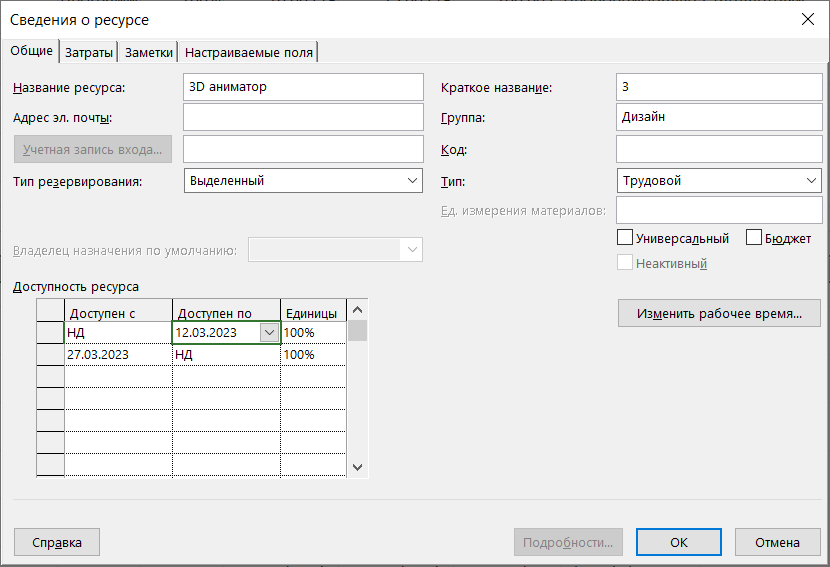
\includegraphics[width=0.7\textwidth]{imgs/task_1_1.png}
	\end{center}
\end{figure}

Его работу в этот период на 20\% выполнял художник-дизайнер, сократив работу по своим задачам до 80\%

\begin{figure}[H]
	\begin{center}
		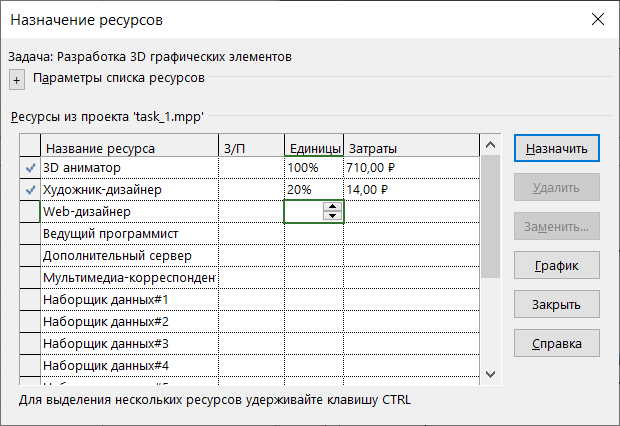
\includegraphics[width=0.7\textwidth]{imgs/task_1_2.png}
	\end{center}
\end{figure}

\begin{figure}[H]
	\begin{center}
		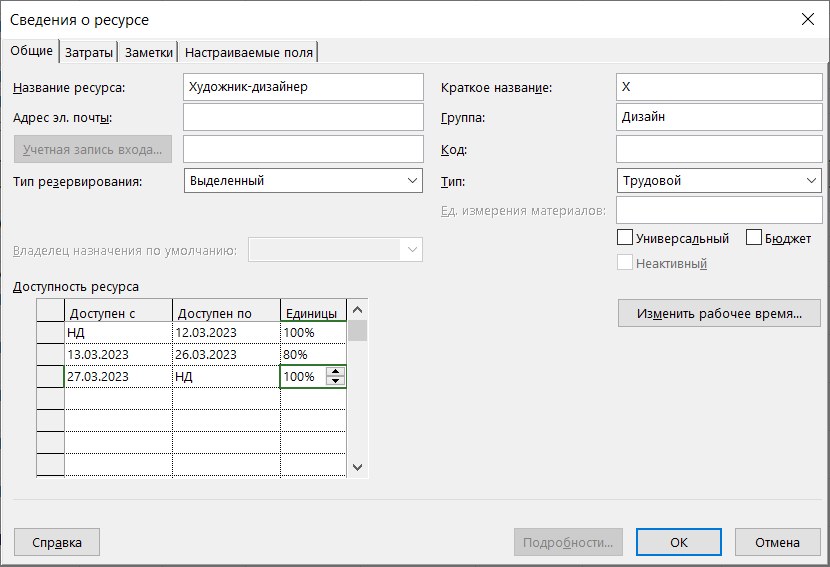
\includegraphics[width=0.7\textwidth]{imgs/task_1_3.png}
	\end{center}
\end{figure}

За совмещение работ в начале апреля художнику–дизайнеру была выплачена премия в размере 500 рублей

\begin{figure}[H]
	\begin{center}
		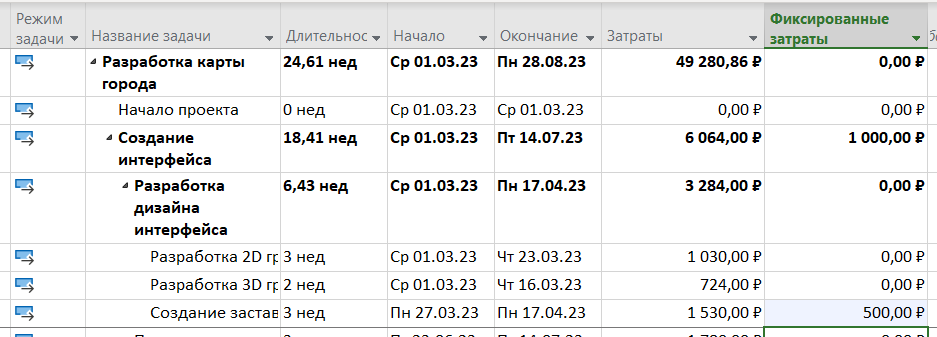
\includegraphics[width=\textwidth]{imgs/task_1_4.png}
	\end{center}
\end{figure}

Задача №7 завершилась на 5 рабочих дней позже

\begin{figure}[H]
	\begin{center}
		
\includegraphics[width=0.7\textwidth]{imgs/task_1_5.png}
	\end{center}
\end{figure}

Фактические трудозатраты на выполнение задачи №15 оказались на 20\% больше

\begin{figure}[H]
	\begin{center}
		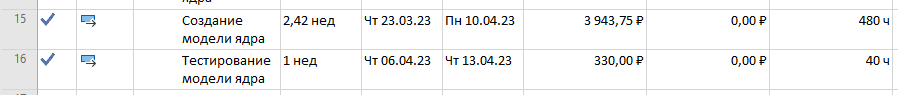
\includegraphics[width=\textwidth]{imgs/task_1_6.png}
	\end{center}
\end{figure}

Задача №17 выполнена на 40\%

\begin{figure}[H]
	\begin{center}
		
\includegraphics[width=0.7\textwidth]{imgs/task_1_7.png}
	\end{center}
\end{figure}

С 12 апреля на 10\% повысилась зарплата мультимедиа корреспондента

\begin{figure}[H]
	\begin{center}
		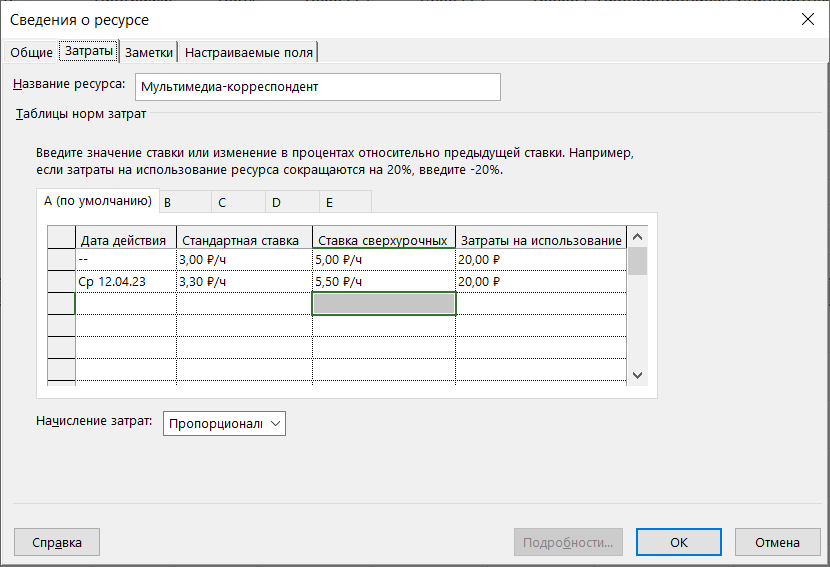
\includegraphics[width=0.85\textwidth]{imgs/task_1_8.png}
	\end{center}
\end{figure}

С 1 апреля отказались от аренды сервера и купили собственный за 3200 рублей

\begin{figure}[H]
	\begin{center}
		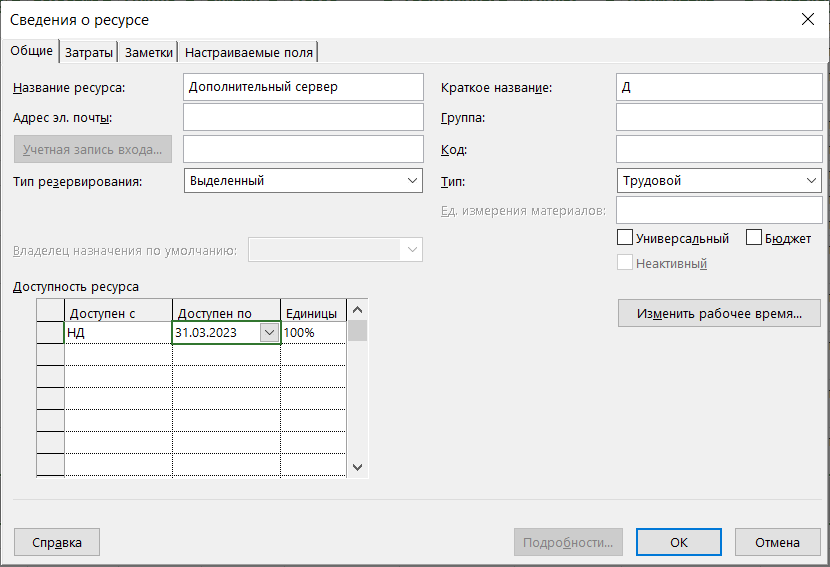
\includegraphics[width=0.85\textwidth]{imgs/task_1_9.png}
	\end{center}
\end{figure}

\begin{figure}[H]
	\begin{center}
		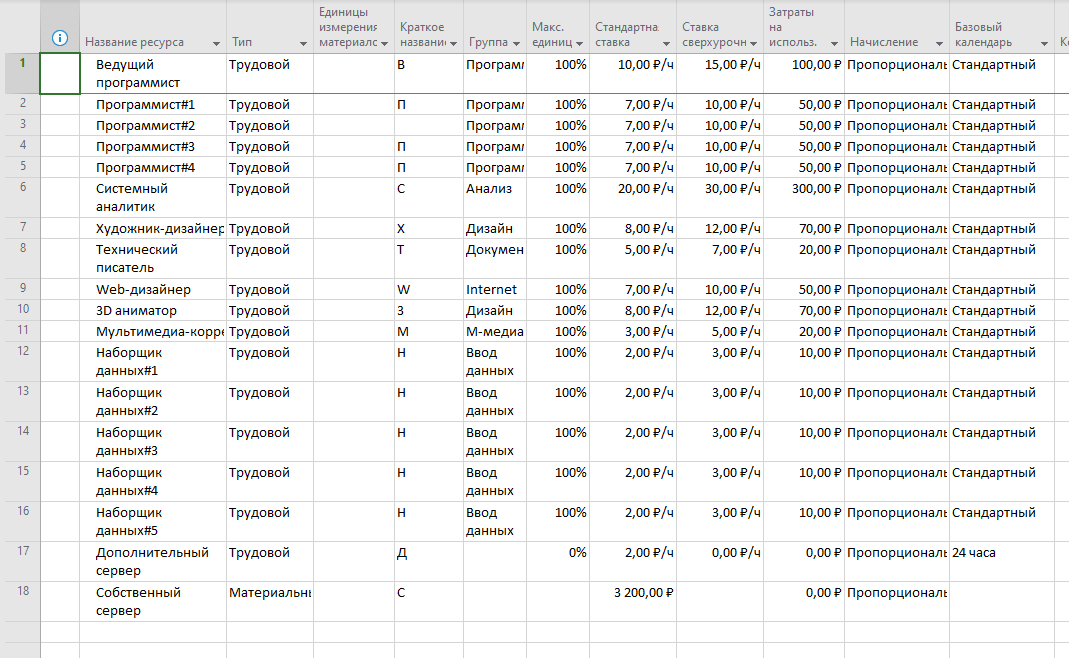
\includegraphics[width=\textwidth]{imgs/task_1_10.png}
	\end{center}
\end{figure}

С 3 апреля в течение двух недель с 10 до 14 часов организуется повышение квалификации для Программистов №1-4

\begin{figure}[H]
	\begin{center}
		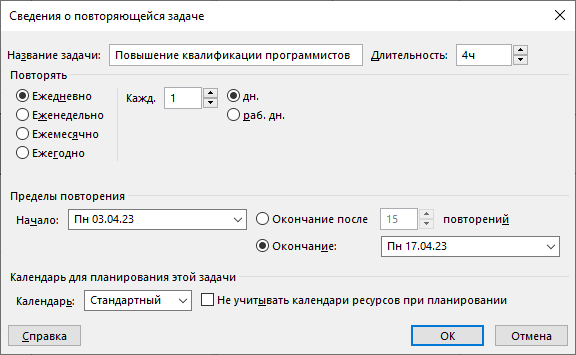
\includegraphics[width=0.85\textwidth]{imgs/task_1_11.png}
	\end{center}
\end{figure}

\begin{figure}[H]
	\begin{center}
		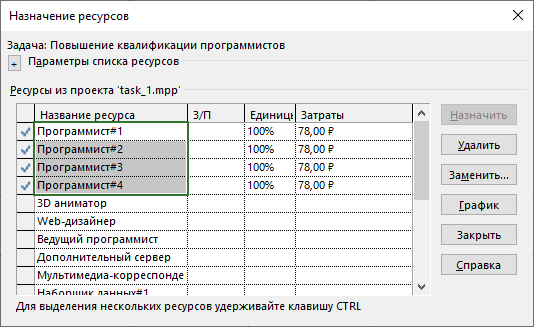
\includegraphics[width=0.85\textwidth]{imgs/task_1_12.png}
	\end{center}
\end{figure}

После завершения обучения их зарплата будет увеличена на 10\%

\begin{figure}[H]
	\begin{center}
		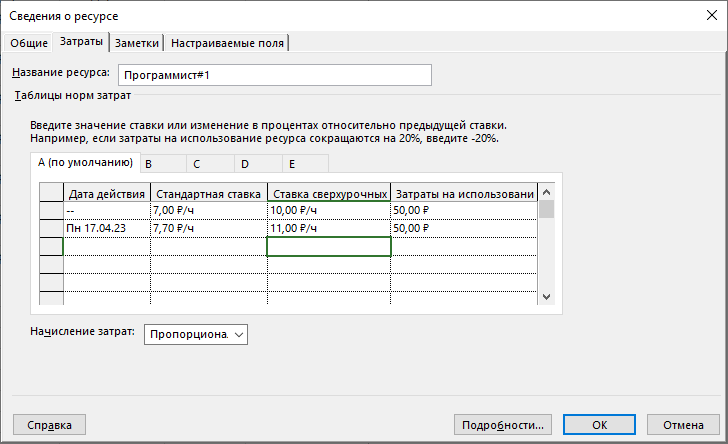
\includegraphics[width=0.85\textwidth]{imgs/task_1_13.png}
	\end{center}
\end{figure}

Для проведения обучения программистов нанят преподаватель с оплатой 700 рублей в неделю

\begin{figure}[H]
	\begin{center}
		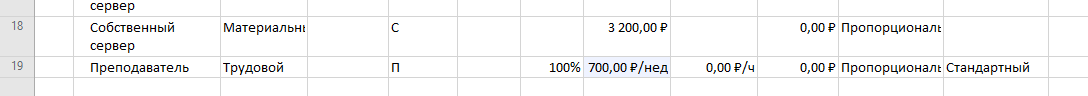
\includegraphics[width=\textwidth]{imgs/task_1_14.png}
	\end{center}
\end{figure}

\begin{figure}[H]
	\begin{center}
		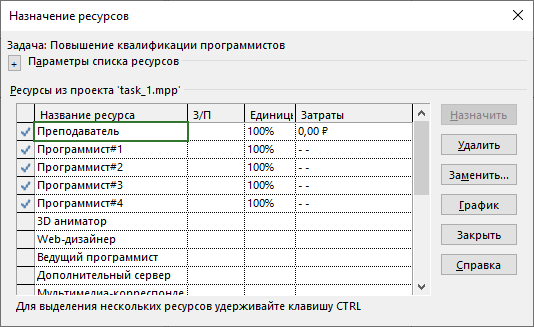
\includegraphics[width=0.7\textwidth]{imgs/task_1_15.png}
	\end{center}
\end{figure}

После внесения фактических данных выяснилось, что проект вышел за рамки бюджета

\begin{figure}[H]
	\begin{center}
		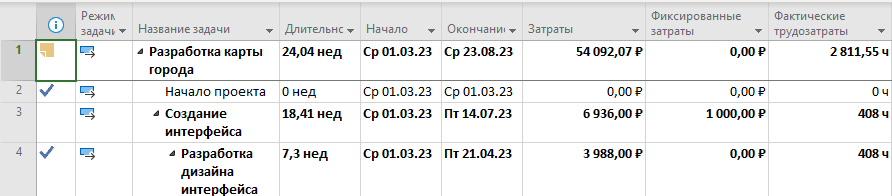
\includegraphics[width=\textwidth]{imgs/task_1_16.png}
	\end{center}
\end{figure}

Также появилась перегрузка ресурсов

\begin{figure}[H]
	\begin{center}
		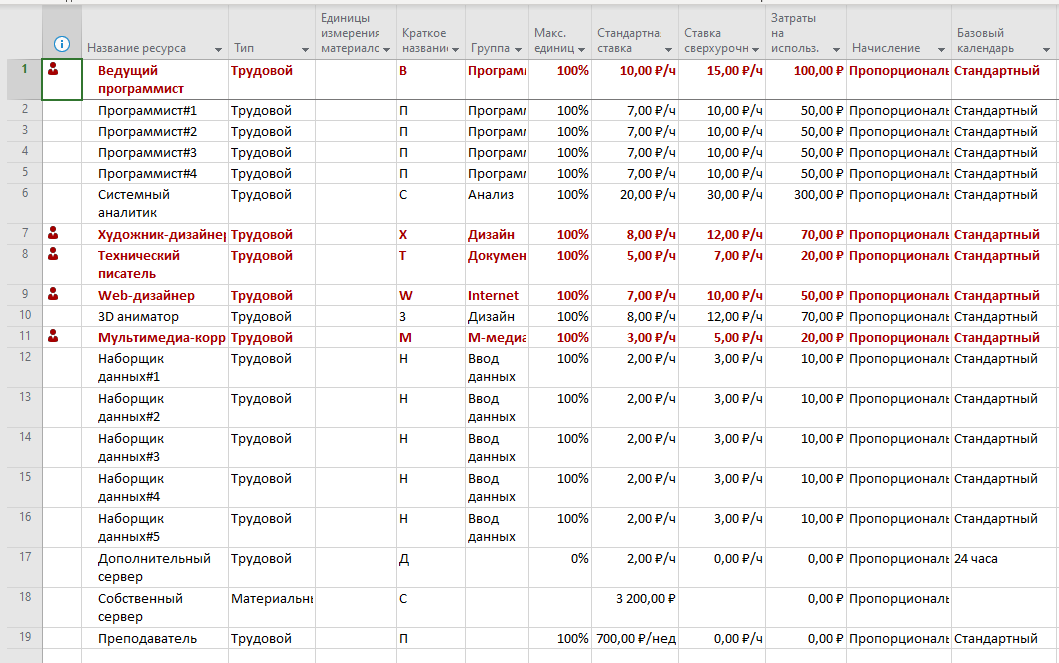
\includegraphics[width=\textwidth]{imgs/task_1_17.png}
	\end{center}
\end{figure}

Расписание

\begin{figure}[H]
	\begin{center}
		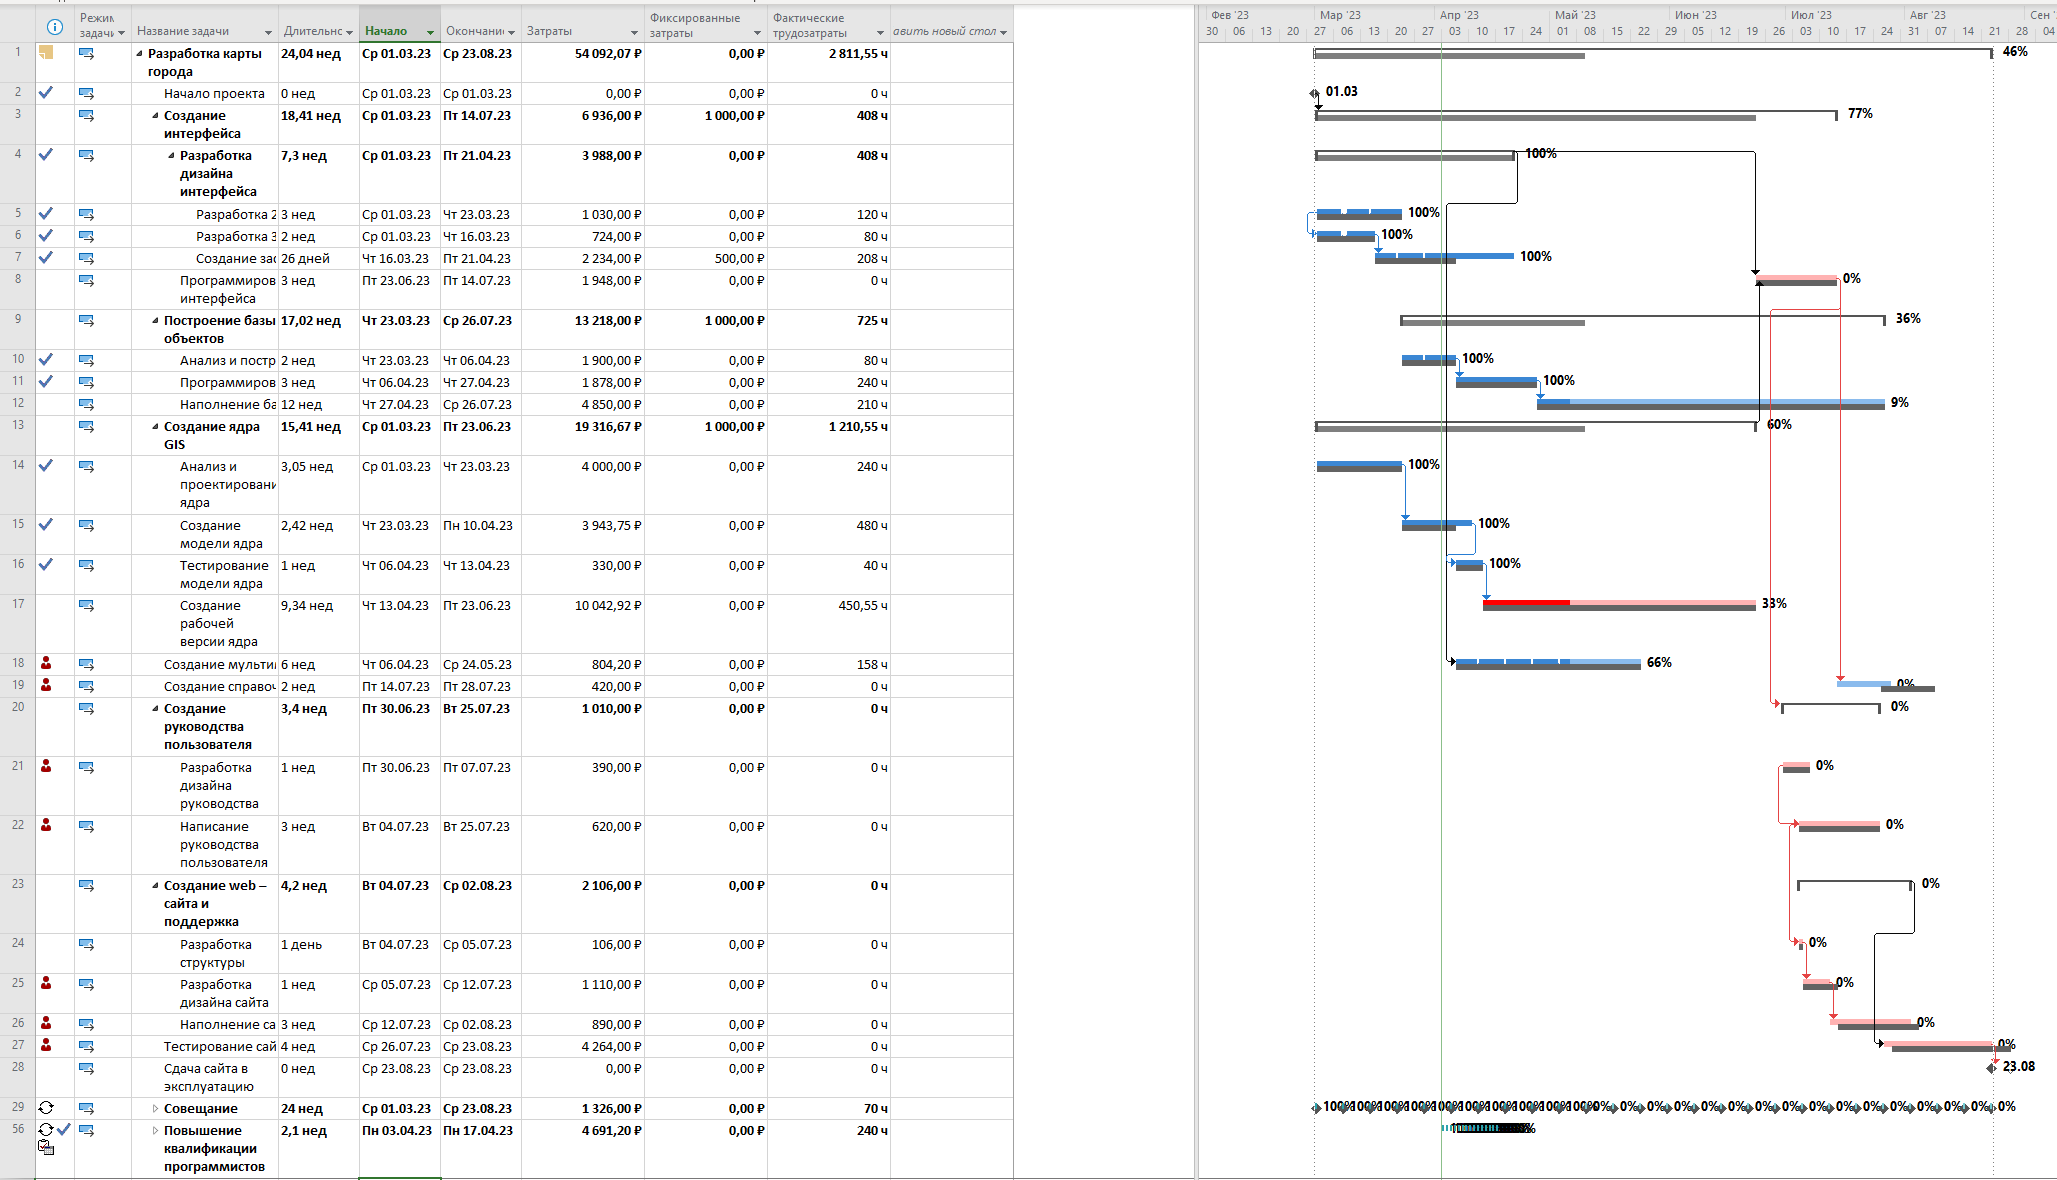
\includegraphics[width=\textwidth]{imgs/task_1_18.png}
	\end{center}
\end{figure}

\section*{Выравнивание}

Уберем у 3 и 4 совещаний заболевшего 3D аниматора:

\begin{figure}[H]
	\begin{center}
		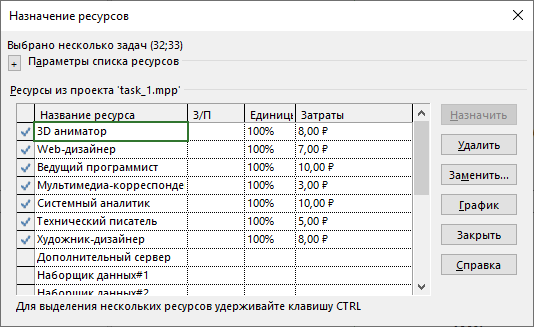
\includegraphics[width=\textwidth]{imgs/task_1_19.png}
	\end{center}
\end{figure}

Произведем выравнивание

\begin{figure}[H]
	\begin{center}
		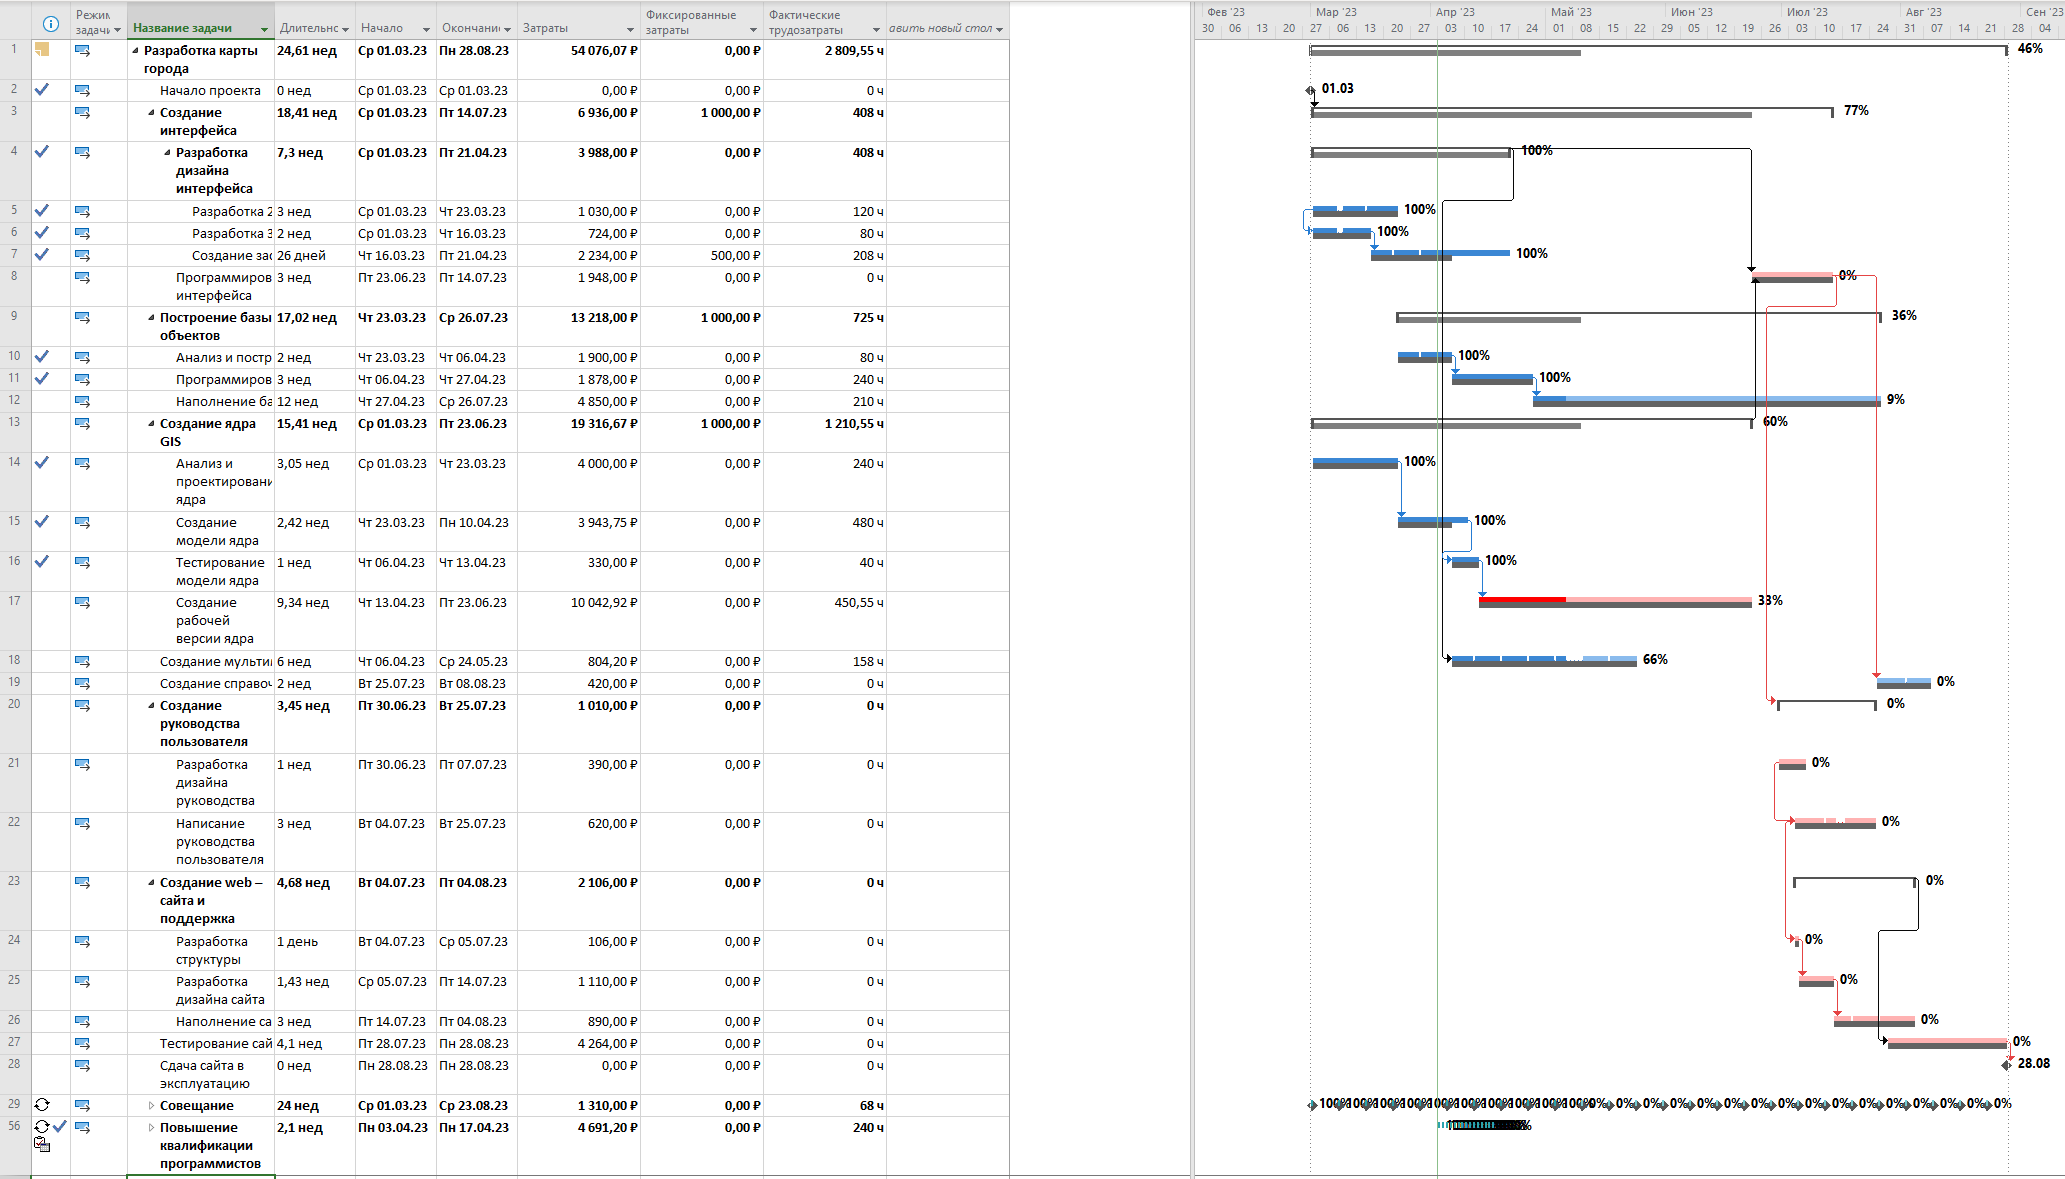
\includegraphics[width=\textwidth]{imgs/task_1_20.png}
	\end{center}
\end{figure}

\section*{Сравнение показателей}

Сроки:

\begin{itemize}
	\item Плановое окончание: 23.08.23
	\item Текущее окончание: 28.08.23
	\item Максимальное окончание: 1.09.23
\end{itemize}

Затраты:

\begin{itemize}
	\item Плановые затраты: 48 766 рублей
	\item Текущие затраты: 54 076 рублей
	\item Бюджет: 50 000 рублей
\end{itemize}

Вывод: перегрузку ресурсов в данных условиях уджалось устранить выравниванием. Срок проекта сдвинулся на 5 дней, что еще допустимо в рамках плана. Также увеличились затраты настолько, что превышают бюджет на 4 076 рублей. Требуется корректировка ресурсов.

\section*{Линия прогресса}

Отобразим линию прогресса проекта

\begin{figure}[H]
	\begin{center}
		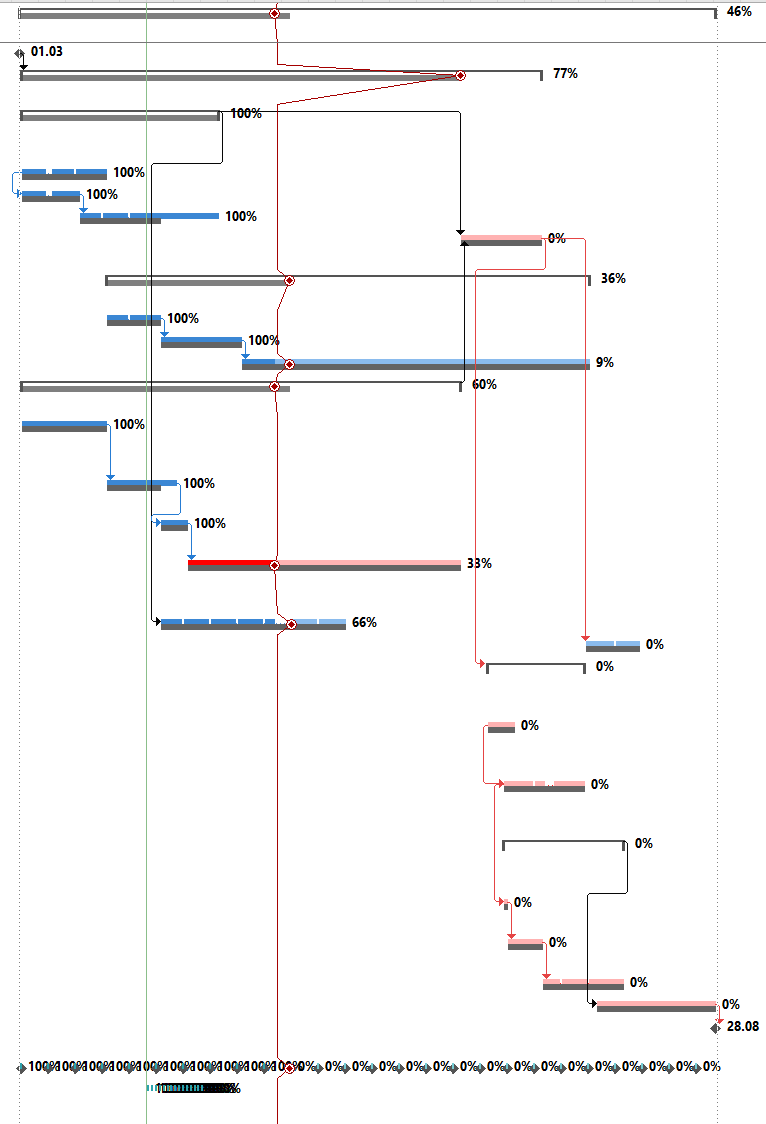
\includegraphics[width=\textwidth]{imgs/task_1_21.png}
	\end{center}
\end{figure}

\section*{Устранение отклонений}

Создание рабочей версии ядра лежит на критическом пути и занимает много времени, ею занимаются все программисты

\begin{figure}[H]
	\begin{center}
		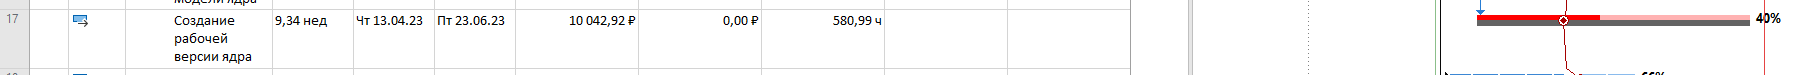
\includegraphics[width=\textwidth]{imgs/task_1_22.png}
	\end{center}
\end{figure}

Добавим программиста-стажера

\begin{figure}[H]
	\begin{center}
		
\includegraphics[width=\textwidth]{imgs/task_1_23.png}
	\end{center}
\end{figure}

И добавим его в две задачи

\begin{figure}[H]
	\begin{center}
		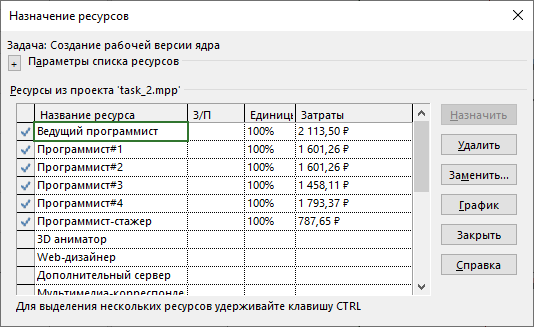
\includegraphics[width=\textwidth]{imgs/task_1_24.png}
	\end{center}
\end{figure}

\begin{figure}[H]
	\begin{center}
		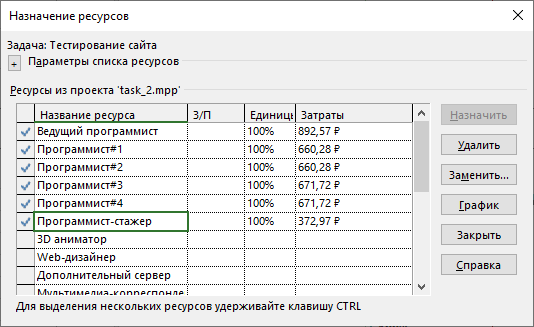
\includegraphics[width=\textwidth]{imgs/task_1_25.png}
	\end{center}
\end{figure}

После чего получим дату окончания 1.08.23 (даже раньше, чем в базовом) и затраты 49 888 рублей

\begin{figure}[H]
	\begin{center}
		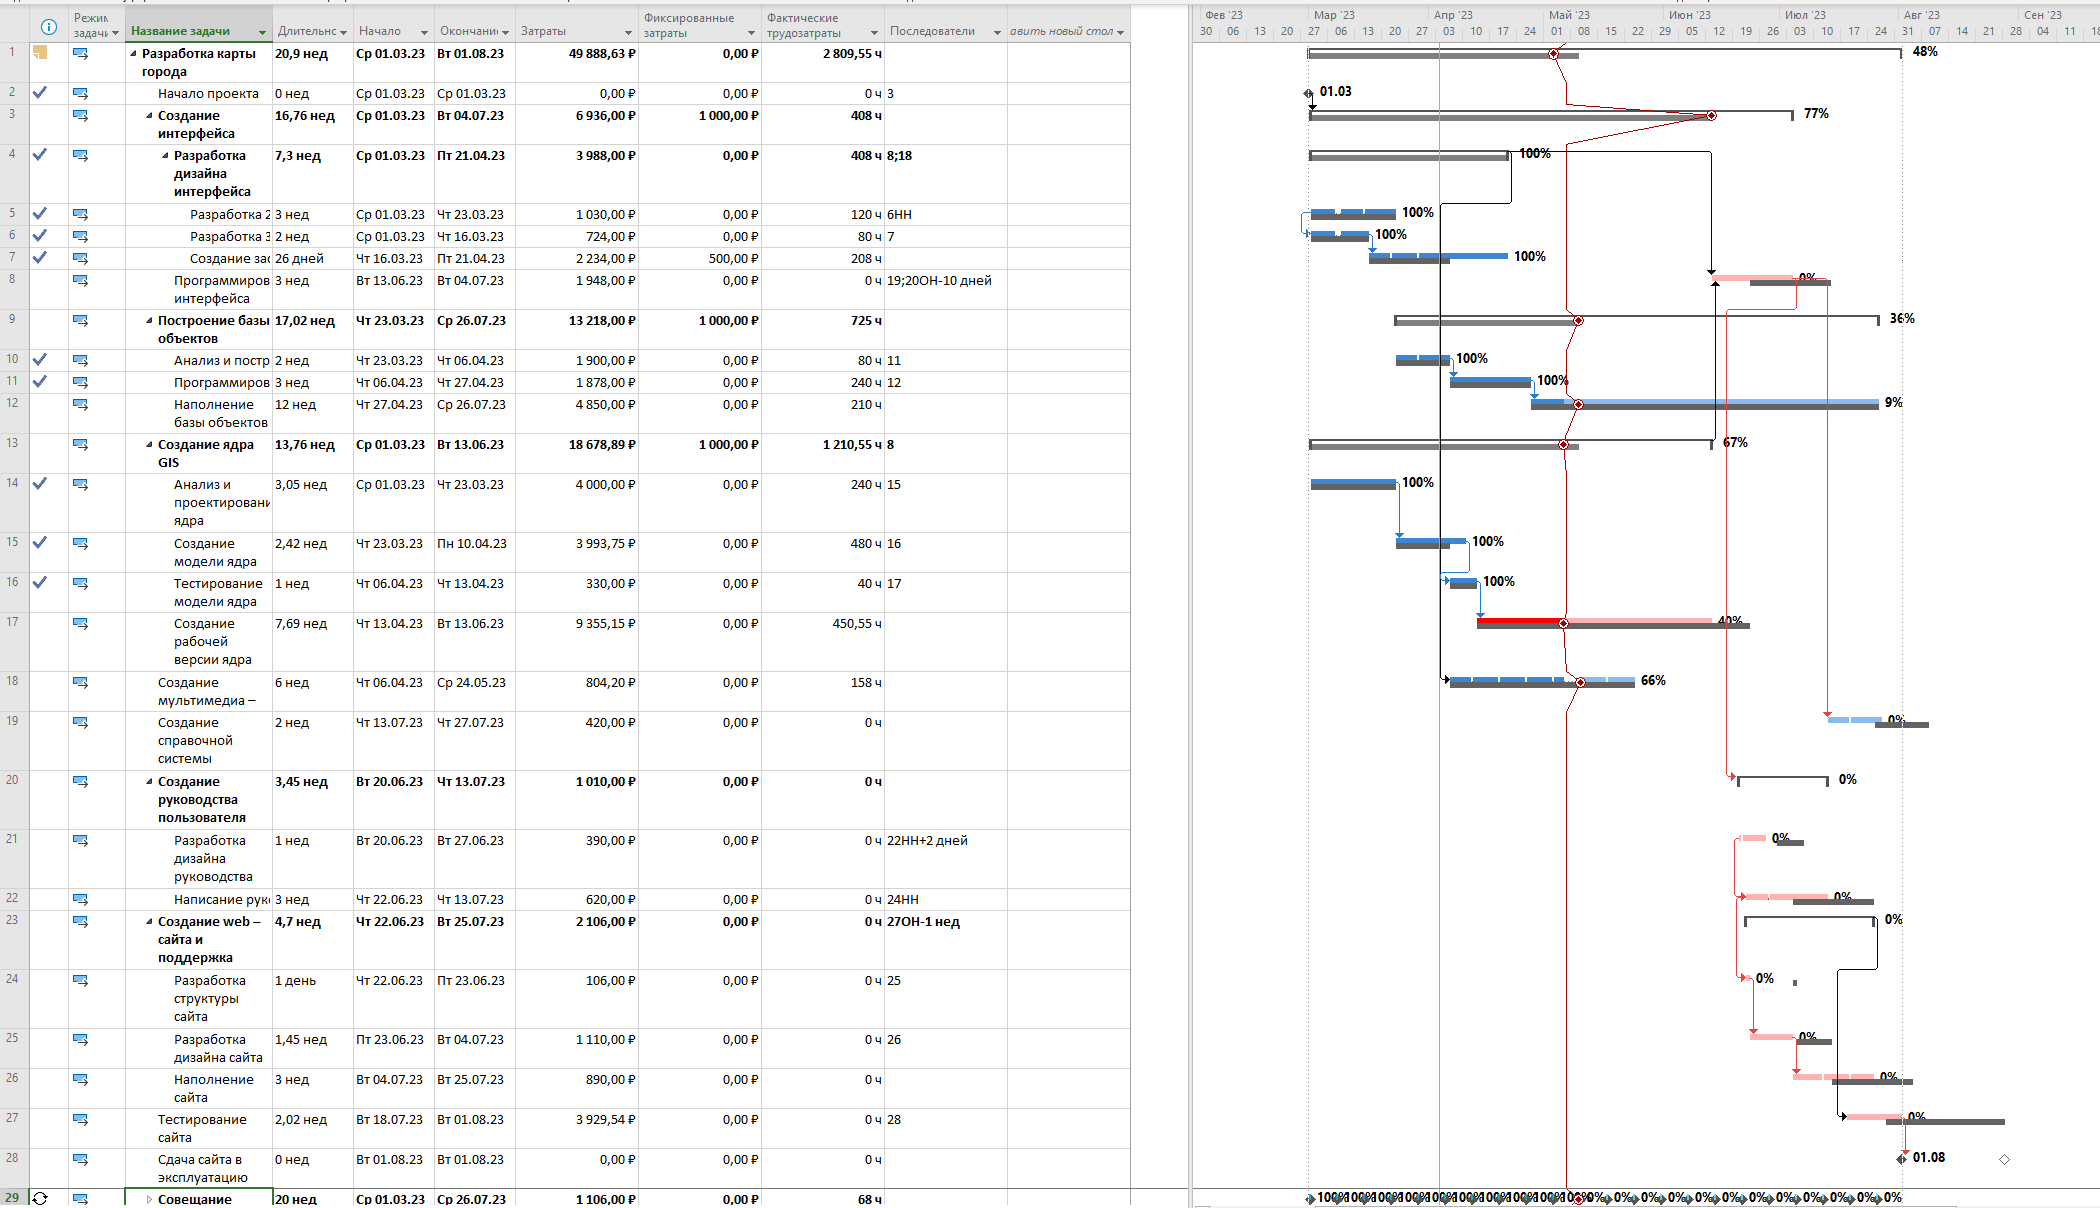
\includegraphics[width=\textwidth]{imgs/task_1_26.png}
	\end{center}
\end{figure}